%%
%% This is file `sample-sigconf.tex',
%% generated with the docstrip utility.
%%
%% The original source files were:
%%
%% samples.dtx  (with options: `all,proceedings,bibtex,sigconf')
%%
%% IMPORTANT NOTICE:
%%
%% For the copyright see the source file.
%%
%% Any modified versions of this file must be renamed
%% with new filenames distinct from sample-sigconf.tex.
%%
%% For distribution of the original source see the terms
%% for copying and modification in the file samples.dtx.
%%
%% This generated file may be distributed as long as the
%% original source files, as listed above, are part of the
%% same distribution. (The sources need not necessarily be
%% in the same archive or directory.)
%%
%%
%% Commands for TeXCount
%TC:macro~\cite [option:text,text]
%TC:macro~\citep [option:text,text]
%TC:macro~\citet [option:text,text]
%TC:envir table 0 1
%TC:envir table* 0 1
%TC:envir tabular [ignore] word
%TC:envir displaymath 0 word
%TC:envir math 0 word
%TC:envir comment 0 0
%%
%% The first command in your LaTeX source must be the \documentclass
%% command.
%%
%% For submission and review of your manuscript please change the
%% command to \documentclass[manuscript, screen, review]{acmart}.

\documentclass[sigconf]{acmart}
%%
%% \BibTeX command to typeset BibTeX logo in the docs
\AtBeginDocument{%
  \providecommand\BibTeX{{%
    Bib\TeX}}}

\setcopyright{acmlicensed}
\copyrightyear{2018}
\acmYear{2018}
\acmDOI{XXXXXXX.XXXXXXX}
\acmConference[Conference acronym 'XX]{Make sure to enter the correct
  conference title from your rights confirmation emai}{June 03--05,
  2018}{Woodstock, NY}
\acmISBN{978-1-4503-XXXX-X/18/06}

\usepackage[ruled,vlined]{algorithm2e}
\SetKwInput{KwGlobalIn}{Global Mem Input}
\SetKwInput{KwSharedIn}{Shared Mem Input}
\SetKwInput{KwSharedOut}{Shared Mem Output}
\SetKwInput{KwGlobalOut}{Global Mem Output}
\SetKwInput{KwConstants}{Constants}

\usepackage{amsmath}
\usepackage{mathtools}
\usepackage{listings}
\usepackage{subcaption}
\usepackage{makecell}
\newcommand{\thomas}[1]{{\footnotesize\color{orange}[Thomas: #1]}}
\newcommand{\john}[1]{{\footnotesize\color{cyan}[John: #1]}}
\newcommand{\raph}[1]{{\footnotesize\color{magenta}[Raph: #1]}}

\begin{document}

\title{Decoupled Fallback: A Portable Single-Pass GPU Scan}

\author{Thomas Smith}
\affiliation{%
  \institution{Google}
  \country{USA}}

\author{Raph Levien}
\affiliation{%
  \institution{Google}
  \country{USA}
}

\author{John D. Owens}
\affiliation{%
  \institution{University of California, Davis}
  \country{USA}}
\additionalaffiliation{%
  \institution{Google}
  \country{USA}
}

\renewcommand{\shortauthors}{Smith et al.}

\begin{abstract}
  We present \emph{Decoupled Fallback}, a method that enables single-pass \emph{Chained-Scans} to run on hardware without \emph{Forward-Progress Guarantees} (FPG) while avoiding deadlock. Additionally, we introduce a tile state representation for \emph{Chained-Scans} that does not rely on 64-bit atomics or memory fences for correctness, along with a subgroup-size-agnostic intra-workgroup implementation. On an FPG-lacking device---Apple M1 Pro (8+2)---\emph{Decoupled-Fallback} achieves near-\emph{memcopy} speeds for inclusive prefix sum in WGPU and realizes the full theoretically expected 50\% speedup over the slower \emph{Reduce-then-Scan} approach. We further demonstrate the resilience of \emph{Decoupled-Fallback} against \emph{unfair} schedulers by emulating blocking at rates of up to 50\%, showing that it maintains superior performance over \emph{Reduce-then-Scan} even under extreme contention.
\end{abstract}

\begin{CCSXML}
  <ccs2012>
  <concept>
  <concept_id>00000000.0000000.0000000</concept_id>
  <concept_desc>Do Not Use This Code, Generate the Correct Terms for Your Paper</concept_desc>
  <concept_significance>500</concept_significance>
  </concept>
  <concept>
  <concept_id>00000000.00000000.00000000</concept_id>
  <concept_desc>Do Not Use This Code, Generate the Correct Terms for Your Paper</concept_desc>
  <concept_significance>300</concept_significance>
  </concept>
  <concept>
  <concept_id>00000000.00000000.00000000</concept_id>
  <concept_desc>Do Not Use This Code, Generate the Correct Terms for Your Paper</concept_desc>
  <concept_significance>100</concept_significance>
  </concept>
  <concept>
  <concept_id>00000000.00000000.00000000</concept_id>
  <concept_desc>Do Not Use This Code, Generate the Correct Terms for Your Paper</concept_desc>
  <concept_significance>100</concept_significance>
  </concept>
  </ccs2012>
\end{CCSXML}

\ccsdesc[500]{Do Not Use This Code~Generate the Correct Terms for Your Paper}
\ccsdesc[300]{Do Not Use This Code~Generate the Correct Terms for Your Paper}
\ccsdesc{Do Not Use This Code~Generate the Correct Terms for Your Paper}
\ccsdesc[100]{Do Not Use This Code~Generate the Correct Terms for Your Paper}

\keywords{Do, Not, Us, This, Code, Put, the, Correct, Terms, for,
  Your, Paper}

\received{20 February 2007}
\received[revised]{12 March 2009}
\received[accepted]{5 June 2009}

\maketitle

\section{Introduction (WIP)}
 (Tell readers we are targeting WebGPU)
 (Speed of light definition here)
\subsection{Goals of a Scan Implementation}
\begin{itemize}
  \item \textbf{Minimal global memory access:} the scan should minimize global memory access to the theoretical minimum of $2n$.
  \item \textbf{Fully saturates global memory bandwidth:} the scan should be capable of fully saturating the global memory bandwidth.
  \item \textbf{Portability:} the scan should be portable across hardware vendors and architectures.
\end{itemize}
Our method retains the best aspects of the \emph{Chained-Scan} architecture, while eliminating the need for forward progress guarantees. It is designed to operate on arbitrary hardware, support arbitrary monoids, process inputs of arbitrary size, and support arbitrary 32-bit and 64-bit data types.
\subsection{Goals}
This work is guided by two main goals:
\begin{enumerate}
  \item \textbf{Portability}: we want to develop a scan implementation that retains the benefits of the \emph{Chained-Scan} architecture but is also suitable for a diverse range of hardware vendors and architectures, including those without FPG or support for 64-bit atomics.
  \item \textbf{Performance}: we aim for near speed-of-light execution to the greatest extent possible allowed by the underlying hardware and programming model.
\end{enumerate}

\noindent
To ground these objectives, we select the WebGPU shading language (WGSL) and the WebGPU standard as our target environment. WGSL is a meta-level shading language which is translated and compiled as necessary for backend graphics APIs---D3D12, Vulkan, and Metal---and as such, WGSL implementations are bound by the minimum capability across all backends. Because WGSL must operate within this limited capability space, it inherently embodies the challenge of portability.

\subsection{Non Goals}
Although our goal is to create a fully portable and highly performant scan implementation, we are constrained by underlying hardware platforms and programming models. As discussed in more detail in \emph{Limits on the Speed-of-Light}, not all architectures offer atomic operations that are sufficiently fast enough or scheduling models that are sufficiently fair enough to attain speed-of-light performance, and thus we cannot guarantee such performance. Although we are cognizant of the risks posed by subgroup divergence, subgroup functions in shading languages do not allow explicit divergence control,\footnote{For example, CUDA allows developers to explicitly provision subgroup functions with a mask of the threads that will participate in them.} placing a solution to subgroup divergence issues outside our scope. Lastly, we do not investigate alternative $O(2n)$ scan architectures beyond \emph{Chained-Scan}.

\subsection{Contributions}
\begin{enumerate}
  \item Decoupled-Fallback
  \item Split-Method
  \item Subgroup-Size Agnostic stuff
\end{enumerate}

\section{Background}
\subsection{Virtualization and Scheduling in the GPU programming model}
Contemporary GPUs are hierarchically organized, massively parallel processors designed to prioritize throughput over latency. (one sentence on thread hierarchy maybe). As comprehensive descriptions of the GPU programming model~\cite{} already exist, we focus on the aspects most relevant to this work: scheduling and synchronization.

\raph{I think "NVIDIA Tesla: A Unified Graphics and Computing Architecture" Lindholm 2008 might be a good choice for the above cite.}

On GPU hardware, scheduling is divided into two levels: a \emph{workgroup} scheduler, which manages kernel launches and maps virtual processors, workgroups, to physical processors, \emph{multiprocessors}, and a \emph{subgroup} scheduler, responsible for selecting which of the currently \emph{occupant} subgroups on a multiprocessor for execution. The GPU programming model virtualizes processors to ensure GPU programs---\emph{kernels}---remain portable across hardware with differing physical resources. Effective virtualization requires \emph{oversubscription}, a programming paradigm where tasks are (over)partitioned in such a way that kernels request more virtual processors than are physically available. As a result, a single multiprocessor may host multiple workgroups simultaneously. However, as a consequence of virtualization, the developer relinquishes control over the order in which workgroups are launched, and once a workgroup begins execution on a multiprocessor, it must run to completion and cannot context switch.

\subsubsection{Inter-Workgroup Barriers}
The virtualization of processors introduces an emergent high-level limitation: the absence of an inter-workgroup barrier. As previously mentioned, workgroups cannot context switch. Although contemporary GPU hardware~\cite{} supports workgroup preemption for prioritizing real-time tasks or managing multi-process workloads, this functionality is deliberately excluded from the GPU programming model. This stems from the prohibitively high overhead in latency and storage associated with moving workgroup contexts on and off chip. In the oversubscription paradigm, where the number of workgroups is theoretically unbounded and typically far exceeds the available multiprocessors, every invocation of such a barrier would necessitate context-switching between all launched workgroups. Due to this high cost, no GPU programming environment furnishes developers with a true unbounded-launch inter-workgroup barrier.\footnote{CUDA recently introduced \emph{Thread Block Cluster} synchronization~\cite{NvidiaCudaGuide}, but it is almost certainly designed to operate within the \emph{Persistent-Thread}~\cite{gupta2012} paradigm, rather than serving as a barrier across an unbounded launch.} Instead, when inter-workgroup synchronization is necessary, developers must rely on kernel launches as synchronization points. However, kernel launches are suboptimal as barriers: they incur overheads due to the heterogeneous nature of the operation, and all execution context is lost between launches.

\raph{I think the above is conflating memory barriers with control barriers. All modern GPU shading languages (since Metal 3.2) provide memory barriers with inter-workgroup (device) scope, but the above paragraph makes more sense interpreted as a control barrier. It might also be worth mentioning that kernel launches do not necessarily sychronize; in Vulkan it's really the pipeline barrier that does the synchronization. I can take a whack at re-writing this.}

\subsubsection{Fairness and Progress}
Because multiple workgroups may reside on a single multiprocessor, two key issues arise at the subgroup scheduling level: \emph{fairness}---how evenly execution resources are distributed among subgroups---and \emph{progress guarantees}---ensuring that subgroups eventually make progress towards termination. However, the term "fairness" is used differently across the literature, leading to potential confusion. Sorensen et al.~\cite{sorensen2016,sorensen2018,sorensen2021}, whose work provides the most comprehensive taxonomy of progress models to date, use "fairness" specifically to describe differing levels of progress guarantees. In contrast, NVIDIA publications~\cite{4523358,Merrill2016} define "fairness" in terms of the distribution of execution resources among subgroups. In this work, we adopt NVIDIA's terminology.

\subsection{The Scan Primitive}\label{sec:the-scan-primitive}
The study of \emph{scan} (\emph{parallel prefix}) networks traces back to the design of carry-lookahead adder circuits and beyond~\cite{5219801,10.5555/1098666}. A scan is typically defined on a monoid \( M \), characterized by a binary reduction operator \( \oplus \) and an identity element \( \varepsilon \). The binary operator \( \oplus \) satisfies the closure property \( \forall a, b \in M, \ (a \oplus b) \in M \) and has an identity element \( \exists \varepsilon \in M, \ \forall a \in M, \ \varepsilon \oplus a = a \). To allow parallelization, \( \oplus \) must be associative, but it is not necessarily commutative, as demonstrated in structures like the \emph{bicyclic semigroup}~\cite{}\footnote{Despite its name, this is a monoid.} and Rabin-Karp's \emph{second fingerprinting method for string matching}~\cite[Section 6]{Karp:1987:ERP}. In a scan, the result at the \( n \)-th element is the reduction of the preceding subsequence of elements. If the subsequence includes the \( n \)-th element, it is called \emph{inclusive}; if it excludes the \( n \)-th element, it is called \emph{exclusive}. The most common scan type is the prefix sum, where \( \oplus \) is addition. For example:
\[
  x = [x_1, x_2, x_3, \dots, x_n] \ \ \ \ \ \ \ y = [1, 1, 1, 1, 1]
\]
\[
  \text{InclusiveScan}(x, \oplus) = [x_1, x_1 \oplus x_2, x_1 \oplus x_2 \oplus x_3, \dots, x_1 \oplus x_2 \oplus \cdots \oplus x_n]
\]
\[
  \text{InclusiveScan}(y, +) = [1, 2, 3, 4, 5]
\]
Due to its significance in circuits and as a fundamental algorithmic primitive, scan has been extensively studied in both electrical engineering and computer science. Harris~\cite{1292373} offers a taxonomy that relates depth, fanout, and wire tracks, while Hinze~\cite{10.1007/978-3-540-27764-4_11} develops an algebraic framework for scans. Snir~\cite{10.1016/0196-67748690003-9} proved that depth $d$ and size $s$ are related by $s + d \ge 2n - 2$, and Fich~\cite{10.1145/800061.808738} proved that among minimum depth scans Ladner-Fischer~\cite{10.1145/322217.322232} networks have optimal size. Blelloch~\cite{Blelloch:1989:SAP} adapted scan to the PRAM model and popularized its use as an algorithmic primitive. Finally, Merrill and Garland~\cite{Merrill2016} provide a review of GPU scan implementations, complementing earlier work by Merrill and Grimshaw~\cite{Merrill2009}.

\subsection{Evolution of Inter-Workgroup Scan Architectures}
Contemporary GPU scans depart from early PRAM-like scans~\cite{Blelloch:1989:SAP} by leveraging the GPU memory hierarchy, which consists of progressively faster but increasingly private tiers. Efficient scans integrate fine-grained intra-workgroup (\emph{local}) strategies in shared memory and registers with coarse-grained inter-workgroup (\emph{global}) strategies in global memory. Given their low arithmetic intensity, local scans are inherently memory-bound, as demonstrated by Merrill and Grimshaw~\cite{Merrill2009}. Consequently, recent scan optimizations have shifted toward refining global strategies, particularly inter-workgroup coordination and synchronization. This section reviews three key approaches---\emph{Scan-then-Propagate}, \emph{Reduce-then-Scan}, and \emph{Chained-Scan}---analyzing their handling of inter-workgroup dependencies and efficiency in minimizing global memory access while maximizing bandwidth utilization.

\subsubsection{Scan-then-Propagate}
Introduced by Sengupta et al.~\cite{10.5555/1280094.1280110}, the \emph{Scan-then-Propagate}~\cite{GPUGems3, Sengupta2011} extends intra-workgroup scans to large inputs by resolving inter-workgroup dependencies in three phases:
\begin{enumerate}
  \item \textbf{Intra-Workgroup (Local) Scan:}  Each workgroup performs an inclusive scan on its assigned work tile, storing local results and reductions in global memory.
  \item \textbf{Spine Scan:} The workgroup reductions, collectively forming the \emph{spine}, are gathered and scanned to compute the \emph{root}, resolving dependencies between work tiles. For large scans, this stage is an insignificant amount of work compared to the first and third.
  \item \textbf{Propagation:} Each workgroup retrieves its portion of the root and adds it to the local scan output.
\end{enumerate}
The absence of inter-workgroup barriers necessitates separate kernel launches for dependency resolution, naturally enforcing this structure. To accommodate arbitrarily large inputs, Sengupta et al. employ recursion, repeatedly applying the three-phase process until the spine fits within a single work tile. Thus, an input of size $n$ and a work tile of size $t$ results in a recursive depth of $\lceil \log_t n \rceil$, and $2\cdot\lceil \log_t n \rceil - 1$ kernel launches. Each recursive step $k$ processes $n/t^k$ tiles, leading to a total of $\sum_{k=1}^{\lceil \log_t n \rceil} n/t^k \approx (n - 1)/(t - 1)$ work tiles over all steps. Since each tile moves $4t$ data ($2t$ local scan, $2t$ propagation), the total global data movement is $O\left(\frac{4t(n - 1)}{t - 1}\right) = O(4n)$.

\subsubsection{Reduce-then-Scan}
If memory bandwidth resources are sufficiently scarce relative to compute, memory-bound algorithms like scan can profit by trading additional computation for reduced memory traffic. This trade-off led to a refinement of the \emph{Scan-Then-Propagate} strategy called \emph{Reduce-Then-Scan}~\cite{10.1145/1375527.1375559, Merrill2009, 10.1109/TPDS.2012.336, 10.5555/2031978.2032029}: by storing only the work tile reduction in global memory during the first phase and performing a redundant scan in the third, it eliminates $n$ global data movement while preserving the three-phase structure:
\begin{enumerate}
  \item \textbf{Work Tile Reduction:} Each workgroup performs a pure reduction on its work tile partition, posting the result to global memory.
  \item \textbf{Spine Scan:} The spine is scanned to produce the root.
  \item \textbf{Intra-Workgroup Scan and Propagation:} Each workgroup performs the local scan on the work tile, incorporating its portion of the root as it writes to global memory.
\end{enumerate}

Merrill and Grimshaw~\cite{Merrill2009} introduced \emph{workgroup raking} to reduce recursion overhead for arbitrarily large inputs. Instead of recursively reducing the spine, the input is partitioned among a fixed number of workgroups, $c$, where $c \geq o$, the total workgroup occupancy. This constrains the spine from a variable, potentially recursive structure to a fixed size $c$, ensuring a recursion depth of at most two. As a result, global memory movement for the spine scan is reduced from $O(n/t)$ to $O(2c)$, and kernel launches are limited to three, yielding a total global memory movement of $O(3n + 4c) = O(3n)$.

Breitbart~\cite{10.5555/2031978.2032029} applied Gupta et al.'s \emph{Persistent-Threads}~\cite{gupta2012} to scan, eliminating kernel launch overheads. Recognizing that raking naturally aligns with this paradigm, Breitbart's method statically \emph{discovers} the workgroup occupancy and launches exactly $o$ kernels. Since multiprocessors are not oversubscribed, workgroups persist for the entire kernel duration, enabling synchronization at an atomics-based inter-workgroup barrier without context switching. While global memory movement remains $O(3n)$, this consolidates the scan into a single kernel, minimizing launch overheads.

\subsubsection{Chained-Scan, Stream-Scan}
First introduced by Yan et al.~\cite{10.1145/2442516.2442539} in \emph{Stream-Scan}, the key innovation of the \emph{Chained-Scan} architecture lies in its hybridization of parallel and serial strategies: achieving parallelism at the intra-workgroup level while minimizing global data movement through serial scan operations at the inter-workgroup level. Instead of using kernel launches as inter-workgroup synchronization points, \emph{Chained-Scans} launch a single kernel that assigns work tiles in a serial order to workgroups, utilizing atomics and bit-packed status flags to ensure coherent views of data. To enforce this serial ordering, work tiles are dynamically assigned using atomic increment operations, rather than arbitrary assignment based on virtualized workgroup indices. This shifts dependency resolution from explicit synchronization via barrier-like structures to implicit synchronization via access order. As a result, each element is read and written exactly once, achieving the theoretical minimum of $2n$.

In any \emph{Chained-Scan}, once a workgroup computes its local scan, it must complete two objectives: communicate its reduction to successor tiles and resolve dependencies by incorporating the reductions of all preceding tiles. This process, which we refer to as \emph{Chained Propagation}, defines the set of inter-workgroup techniques that facilitate dependency resolution. In \emph{StreamScan}, these two objectives are combined into a single phase, where each workgroup waits for its immediate predecessor to complete, ingests the predecessor's reduction, and posts the resulting \emph{inclusive} reduction for its immediate successor to consume. This approach depends on a \emph{forward progress guarantee} of the GPU's execution model. Given such a guarantee, the predecessor will eventually produce a result and broadcast it. On devices lacking such a guarantee, the workgroup may wait indefinitely, resulting in deadlock.

While \emph{StreamScan} successfully reduces per-element device memory accesses to two, it does not consistently saturate global memory bandwidth, preventing it from achieving speed-of-light performance. This limitation arises because a workgroup in \emph{StreamScan} cannot post its reduction to global memory until it has received the result of its immediate predecessor. While this results in efficient $O(n/t)$ communication of reductions, and $O(2n+ n/t)= O(2n)$ total data movement, the sequential dependency creates a bottleneck that limits performance to the rate at which reductions propagate through device memory. Although this can be mitigated by increasing the size of the work tile, limited on-chip resources preclude scaling the tile size indefinitely. Moreover, this approach is unsuitable for a portable environment, as excessively large work tiles risk reducing occupancy on less capable hardware.

\subsubsection{Chained-Scan, Decoupled-Lookback}
Introduced by Merrill and Garland, the \emph{Decoupled-Lookback} technique refines \emph{Chained Propagation} by separating reduction communication from dependency resolution, mitigating bottlenecks caused by propagation latency. In this approach, each workgroup posts its local reduction to global memory and then performs a \emph{lookback}---a serial traversal backward along the spine---to compute its inclusive reduction. Work and memory accesses are constant-bounded to the workgroup occupancy $o$ by posting the inclusive reduction after the lookback. However, granting each workgroup control over its dependency resolution does not eliminate reliance on \emph{progress guarantees}, as workgroups must still spin on tiles that have yet to post their reductions, risking deadlock.

Although \emph{Decoupled-Lookback} increases global memory access during the propagation phase to $O(o(n/t))$, the serial ordering of work tile processing confines spine memory accesses to a roughly $o$-width sliding window, making them highly likely to be cache-resident. As a result, the additional global memory traffic along the spine introduces negligible overhead. With total global memory movement of $O(2n+o(n/t))= O(2n)$, \emph{Decoupled-Lookback} achieves full utilization of device memory bandwidth and delivers speed-of-light performance without the work tile size tuning required by \emph{Stream-Scan}.

\subsection{Ideal Scan Architecture}
\emph{Chained Scan} and \emph{Reduce then Scan} represent two contrasting paradigms in scan design: one embraces oversubscription and dynamic scheduling, while the other relies on a fixed-launch model with explicit control over occupancy. By avoiding explicit inter-workgroup synchronization, \emph{Chained-Scan} naturally aligns with the oversubscription paradigm, allowing the workgroup scheduler to dynamically manage occupancy. In contrast, \emph{Reduce-Then-Scan} employs workgroup raking, which mandates explicit occupancy control and, in some cases, inter-workgroup synchronization.

\raph{I'm having trouble with the above paragraph. By my read, Reduce-Then-Scan avoids inter-workgroup synchronization other than the pipeline barriers between kernel launches. Chained-Scan and Decoupled-Lookback both rely on inter-workgroup synchronization. Not sure why the "in some cases" qualifier either; seems to me you need synchronization except in the trivial case the entire array fits in one workgroup.}

Fixed-launch approaches, such as those used in \emph{Reduce-Then-Scan}, introduce several challenges. They require either careful tuning of workgroup launch sizes across different architectures or an occupancy discovery mechanism, which is nontrivial to implement. For example, the workgroup occupancy discovery technique proposed by Sorensen et al.~\cite{sorensen2016} relies on memory fences—unsupported in WebGPU—making it infeasible in certain environments.\footnote{Our implementation includes a fenceless occupancy discovery method suitable for WebGPU, but its description is beyond the scope of this work.}

\raph{"Fixed launch" means launching a fixed number of workgroups and having each workgroup process multiple blocks, generally total blocks / num workgroups? I think I get the argument here but it's more subtle and not an inherent problem with RTS. You make a choice: either you do fixed launch and have to tune, *or* you can do a fixed number of blocks per workgroup, but in the latter case you need to need vary the number of dispatches based on total number of blocks. That's annoying but not a showstopper.}

Hardware-level considerations further underscore the limitations of fixed-launches. On GPUs where the global memory data cache is indexed by physical addresses---and therefore requires lookups in \emph{translation lookaside buffers} (TLBs)---fixed-launches can lead to performance degradation due to cache thrashing. This issue occurs when task sizes are large enough that each workgroup accesses its own unique page entry, and the device lacks sufficient TLB coverage to support the memory access patterns of all workgroups. Although this behavior typically does not manifest with simple monoids, more complex monoids with \emph{struct-of-array} memory access patterns---or applications like radix sorting, where the scattering phase of each pass results in $radixDigits \cdot o$ unique memory locations---may experience significant performance degradation.

Given these constraints, oversubscription and \emph{Chained Scan} emerge as the more portable and preferred architecture. By leveraging the workgroup scheduler, \emph{Chained-Scan} dynamically distributes work across architectures without requiring developer intervention. Furthermore, its single-kernel design and serial ordering make it suitable for \emph{in-situ} operations, benefiting applications such as data deduplication, sparse data compaction, error correction, and interval merging.

However, while \emph{Chained-Scan} with \emph{Decoupled Lookback} appears to be the ideal scan architecture in both theoretical and practical terms, it has a critical limitation: its reliance on a forward-progress guarantee. While NVIDIA GPUs provide this guarantee, data collected by Sorensen et al.~\cite{sorensen2021} shows that Apple’s M-series and ARM GPUs do not. Without forward progress guarantees, \emph{Chained-Scan} is not merely inefficient---it risks indefinite deadlock, causing the application to freeze and rendering the kernel unable to terminate, requiring external intervention to recover.

\subsection{Why does \emph{Chained-Scan} Rely on Forward-Progress Guarantees?}
A \emph{forward-progress guarantee} (FPG) ensures that all occupant subgroups (from possibly different workgroups) eventually make progress toward termination, preventing indefinite starvation. Sorensen et al.~\cite{sorensen2018,sorensen2021} provide the most comprehensive analysis of GPU schedulers, classifying \emph{Chained-Scan} as FPG-reliant. However, their work primarily focuses on formalizing progress models rather than their direct application to specific algorithms.

\raph{I think the deep-dive into the nature of deadlock can be trimmed back here, but chatting with John, such editing for concision can be done later, when we have a better sense about page count.}

The challenges faced by \emph{Chained-Scan} resemble the \emph{Dining Philosophers Problem}, where competing tasks share limited resources, risking deadlock. Coffman et al.~\cite{10.1145/356586.356588} define four conditions necessary for deadlock:
\begin{enumerate}
  \item \textbf{Mutual Exclusion}: Tasks claim exclusive control of resources they require.
  \item \textbf{Resource Holding}: Tasks hold acquired resources while waiting.
  \item \textbf{No Preemption}: A resource cannot be removed from a task before completion.
  \item \textbf{Circular Dependency}:
        \begin{enumerate}
          \item Dependency Relationships: A dependency exists such that each task holds one or more resources that are required by proceeding tasks.
          \item Circular Ordering: A circular chain of tasks exists.
        \end{enumerate}
\end{enumerate}
Applying this schema to \emph{Chained-Scan}, workgroups correspond to "tasks" and work-tile reductions to "resources." Conditions 1–3 hold due to the one-to-one mapping of work tiles to workgroups and the constraints of the GPU programming model. Condition 4a is satisfied by the inter-tile dependencies, leaving condition 4b---\emph{circular ordering}---as the key concern.

Although the serial assignment of work tiles ensures that predecessor tiles are scheduled or completed, it does not guarantee their reductions will be available when a workgroup begins \emph{Chained Propagation}. This uncertainty arises because workgroups are scheduled \emph{individually}, meaning a predecessor may not have had the opportunity to compute and post its reduction. In such cases, the dependent workgroup spins, consuming execution resources while waiting. Because workgroups may share execution resources by being co-resident on the same multiprocessor\john{Question, and maybe this is worth a footnote. What if we guaranteed that no multiprocessor ever had more than one workgroup scheduled to it, say by always allocating the maximum amount of workgroup memory? Of course there would be performance issues. But does that solve the problem? Or do we descend into an analogous issue with subgroup scheduling?}, without FPG, the scheduler may indefinitely prioritize the spinning workgroup over its predecessor, preventing progress and creating a circular dependency, satisfying condition 4b and resulting in deadlock.

\raph{Answering John's question here. Short answer no. One mental model that would illustrate this is a workgroup being preempted from a multiprocessor for system reasons, for example to perform compositing for scanout. I brought this up with a GPU engineer and they said this wasn't actually the reason for lack of FPG on their hardware, but wasn't able to explain the true story for proprietary reasons. In any case, while I am fine to a large extent talking operationally about scheduling etc, at the end of the day you need a formal model that tells you which computations will terminate. That's what Tyler's work is about and I think it's best to cite it and not try to re-litigate it, especially in oversimplified form. Also, taking another look at "Specifying and Testing," I notice that they use "livelock" but not deadlock to describe situations where system progress depends on FPG. I'm not finding a cite for this now, but if memory serves, a deadlock condition is one in which no progress is possible under *any* scheduling condition, while in livelock there is some scheduler condition that could resolve the livelock, but it is not resolved under all such conditions.}

For example, consider a scan operation requiring two workgroups on a GPU with a single multiprocessor. Both workgroups are co-resident, but the multiprocessor has only one scheduling unit, which lacks FPG\@. Both workgroups launch and acquire their respective work tiles. The workgroup responsible for \emph{Work Tile 1} finishes first and begins spinning, repeatedly querying the memory address for the reduction of \emph{Work Tile 0}. However, because the scheduler lacks FPG, it continues scheduling \emph{Work Tile 1}, leaving \emph{Work Tile 0} starved and unable to complete its reduction. As a result, \emph{Work Tile 1} spins indefinitely, eventually triggering \emph{timeout detection and recovery}\footnote{\emph{Timeout detection and recovery} is} (TDR) and crashing the host program.

\subsection{Why is reliance on Forward Progress Guarantees a Portability Problem?}
The absence of FPG in key hardware segments poses a critical challenge for developers. Our testing shows that, at best, running \emph{Chained-Scan} without FPG results in severe performance degradation, and at worst, risks TDR and program crashes.
\begin{figure}
  \centering
  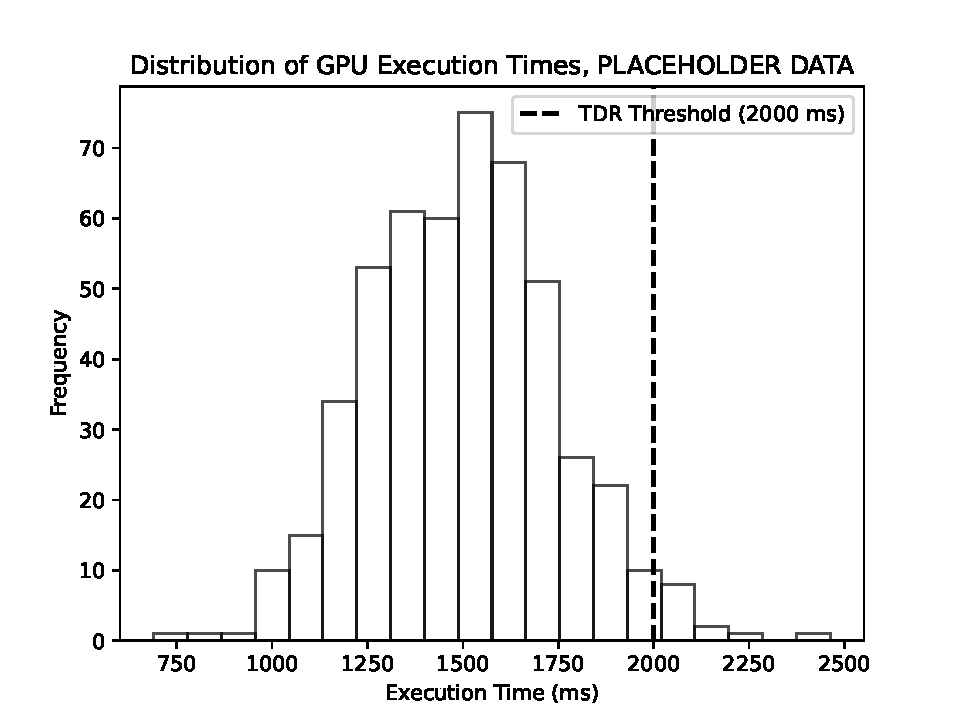
\includegraphics[width=\linewidth]{graphics/Figure_1.pdf}
  \caption{Execution times of \emph{Decoupled-Lookback (PLACEHOLDER DATA)}}
\end{figure}
Exacerbating this issue, no major graphics API provides a mechanism to query FPG support. This lack of transparency forces developers to design algorithms without knowing whether critical guarantees are available on the target hardware. In shader environments, where cross-platform portability is essential, this uncertainty compels a fallback to older, less efficient strategies like \emph{Reduce-Then-Scan}, sacrificing performance for broader compatibility.

\subsection{Earlier Attempts at Portability}
Our first attempt \raph{we'll add the cite post-review} at implementing a \emph{Decoupled-Lookback} scan without relying on FPG was \emph{Scalar Fallback}. Each time a workgroup spins waiting on the reduction from a preceding tile, it advances a \emph{fallback} operation by processing one scalar element from that tile. This eliminates the possibility of deadlock because the number of such operations is bouded; the wait will eventually terminate, possibly at the expense of doing redundant work.

\emph{Scalar Fallback} suffers from two primary inefficiencies. First, the fallback reduction is performed serially by a single thread, progressing only when the lookback thread performs a waiting spin. This results in a $t$-sized blocking tile requiring $t$ spins to complete. Second, once the fallback completes, the lookback thread does not post its result to device memory, forcing every blocked workgroup to redundantly recompute the fallback. While \emph{Scalar Fallback} achieved speed-of-light performance on hardware with FPG and executed correctly without it, its performance on the latter was inferior to \emph{Reduce then Scan}.

\section{Decoupled Fallback}
\emph{Decoupled Fallback} addresses both inefficiencies. The key advance is to utilize the parallelism available in the workgroup to perform the fallback computation, rather than performing it sequentially. To do so requires nontrivial coordination within the workgroup, given that the \emph{Chained-Propagation} logic is performed by a single thread\thomas{Is this clearer as "single subgroup?"}.

\begin{algorithm}
  \small
  \SetAlgoLined
  \KwGlobalIn{%
    $\textit{in}[]$,
    $\textit{out}[]$,
    $\textit{spine}[]$,
    $\textit{tileBump}$,
  }
  \KwSharedIn{%
    $\textit{wg\_partials}[]$,
    $\textit{wg\_fallback}[]$,
    $\textit{wg\_prev\_reduction}$,
    $\textit{wg\_broadcast}$,
    $\textit{wg\_control}$,
  }
  \KwGlobalOut{$\textit{out}[]$ inclusive scan of $\textit{in}[]$}
  \KwConstants{Vectors per thread $\textit{p}$}

  \If{$\textit{threadid} = 0$}{
    $\textit{wg\_broadcast} \gets \textnormal{atomicAdd}(\&\textit{tileBump}, 1)$\;
    $\textit{wg\_control} \gets \textnormal{LOCKED}$\;
  }
  \textbf{barrier()}\;

  $\textit{part\_id} \gets \textit{wg\_broadcast}$\;

  \textit{local\_vectors}: $\textnormal{array}\langle \textnormal{vec4}\langle u32\rangle, \textit{p} \rangle$\;

  \textbf{Load}($\textit{in}$, $\textit{part\_id}$, \textit{local\_vectors})\;
  \textbf{SubgroupRake}(\textit{local\_vectors})\;

  \If{$\textnormal{highestRankLane}(\textit{threadid})$}{
    $\textit{wg\_partials}[\textit{subgroup\_id}] \gets \textit{local\_vectors}[\textit{p} - 1]$\;
  }
  \textbf{barrier()}\;

  \textbf{WorkgroupWideScan}($\textit{wg\_partials}$)\;
  \textbf{barrier()}\;

  \tcp{Chained Propagation, Decoupled Fallback}
  \While{$\textit{wg\_control} = \textnormal{LOCKED}$}{
    \textbf{Lookback}($\textit{spine}$, $\textit{wg\_prev\_reduction}$, $\textit{wg\_control}$)\;
    \textbf{barrier()}\;

    \If{$\textit{wg\_control} = \textnormal{LOCKED}$}{
      \textbf{FallbackReduce}($\textit{in}$, $\textit{wg\_fallback}$)\;
      \textbf{FallbackInsertionAttempt}($\textit{spine}$, $\textit{wg\_fallback}$, $\textit{wg\_prev\_reduction}$, $\textit{wg\_control}$)\;
      \textbf{barrier()}\;
    }
  }

  \textbf{Write}($\textit{out}$, $\textit{part\_id}$, \textit{local\_vectors}, $\textit{wg\_partials}$, $\textit{wg\_prev\_reduction}$)\;

  \caption{High-Level Scan Kernel}
\end{algorithm}

To optimize the fallback operation, we employ three strategies. (1) First, a shared memory \emph{control flag} enables threads performing the lookback to signal the entire workgroup when a fallback is necessary. (2) Next, we limit the number of spins a thread can perform while waiting on a tile; exceeding this threshold triggers a fallback. While this approach risks redundant fallbacks---since a late tile is indistinguishable from a genuinely blocking one---exposing the maximum spin count as a tunable parameter helps minimize false positives. \john{I can see it is sensible to have a maximum spin count but I do not see how the action of exposing the maximum spin count to the programmer minimizes false positives.} (3) Finally, after completing a fallback, the workgroup attempts to post the reduction result of the blocking tile, preventing redundant fallbacks by subsequent workgroups.

\raph{To address John's comment: increasing the spin count reduces false positives; a false positive can be defined as the preceding tile posting the result late, meaning that there is some spin count for which it would proceed. However, it also delays progress in the true positive case. The deeper way to talk about this is to engage the cost model, which is done to some extent in the paragraph below. The cost of a false positive includes increased memory traffic and also compute opportunity cost of other workgroups which can be scheduled on the same multiprocessor. Indeed, with sufficient occupancy the cost of a workgroup spinning (or making scalar progress) is minimal. So optimal performance really depends on the *distribution* of spin counts. I put all this in a comment but think we can say it in the paper.}

The viability of \emph{Decoupled-Fallback} relies on the same cache locality properties as \emph{Decoupled-Lookback}. Since no subgroup scheduler is perfectly fair, all hardware inherently has a natural fallback rate $f$\!, independent of FPG, due to \emph{false-positive} fallback operations. As a result, memory bandwidth usage increases (and we expect throughput to decrease) by $O(fn)$ to $O((2 + f)n)$. However, just as serial ordering confines spine memory accesses within an $o$-width sliding window, scan input accesses are likewise constrained to an $ot$-width window, increasing their likelihood of residing in cache. As we later empirically demonstrate(Simulated Blocking Section), this cache residency significantly reduces memory access costs, making fallback operations predominantly compute-bound when reducing a blocking tile. Since pure reduction has minimal overhead, throughput approaches $O(2n)$ on most devices.

\section{Implementation}
At a high level, our algorithm follows a five-phase construction:
\begin{enumerate}
  \item[(0)] \textbf {Initialization}: The first thread in the workgroup atomically acquires its work-tile by atomically incrementing a value in global memory.
  \item \textbf{Load Phase}: Each thread loads $p$ vectors, consuming the input in a subgroup-blocked ordering. For a subgroup size $s$ and vector size $v$, each subgroup processes a contiguous block of size $s \cdot p \cdot v$.
  \item \textbf{Subgroup-Rake}: Each thread scans its vectors privately, then joins $p$ raking Kogge-Stone~\cite{} subgroup scans,
        allowing the subgroup-block scan to remain barrier-free and in registers. The subgroup-block reduction is then posted to shared memory. For a workgroup of size $w$, subgroup-raking reduces the size of the local spine to $w/s$.
  \item \textbf{Workgroup-Wide Scan}: The workgroup collectively performs a scan across the subgroup partial reductions, writing the results back to shared memory upon completion.
  \item \textbf{Chained Propagation, Decoupled Fallback}: The first subgroup in the workgroup performs a lookback operation to acquire the reduction result of all previous workgroups, engaging in fallback operations as necessary. Once completed, this subgroup posts the results to shared memory for the workgroup to consume.
  \item \textbf{Write Phase}: Each subgroup incorporates the results from the workgroup-wide scan and lookback operation to produce and write out the correct output.
\end{enumerate}
Phase 0 ensures that the work tiles are consumed in serial order. Phases 1, 2, 3, and 5 comprise the intra-workgroup scan, following a \emph{Scan-then-Propagate} strategy. Phase 4, \emph{Decoupled-Fallback}, is responsible for managing all inter-workgroup dependencies. As our loading and writing phase are typical of scan kernels, we focus here on our portability-specific adaptations.

\begin{algorithm}
  \small
  \SetAlgoLined
  \KwSharedIn{ Array of subgroup partial reductions $\textit{x}$ }
  \KwSharedOut{ Inclusive-scanned $\textit{x}$ }
  \KwConstants{ Workgroup Size $\textit{W}$, Subgroup Size $\textit{S}$ }

  $\textit{spine\_length} \gets \textit{W} / \textit{S}$\;
  $\textit{alignment} \gets 1 << \text{divRoundUp}(\log_2(\textit{spine\_length}), \log_2(\textit{S})) \cdot \log_2(\textit{S})$\;

  $\textit{stride} \gets 1$\;
  $\textit{top\_offset} \gets 0$\;

  \ForEach{$\textit{thread\_id}$ \textbf{in} $\textit{W}$ \textbf{in parallel}}{
    \For{$\textit{j} \gets \textit{S}$ \KwTo $\textit{alignment}$ \textbf{with} $\textit{j} \gets \textit{j} \cdot \textit{S}$}{
      \tcp{Brent-Kung Upsweep}

      $\textit{step} \gets \textit{spine\_length} / \textit{stride}$\;

      \If{$\textit{thread\_id} < \textit{step}$}{
        $\textit{temp} \gets \text{subgroupInclusiveScan}(\textit{x}[\textit{thread\_id} + \textit{top\_offset}])$\;
        $\textit{x}[\textit{thread\_id} + \textit{top\_offset}] \gets \textit{temp}$\;
        \If{$\text{\normalfont highestRankLane}(\textit{thread\_id})$}{
          $\textit{x}[(\textit{thread\_id} / \textit{S}) + \textit{step} + \textit{top\_offset}] \gets \textit{temp}$\;
        }
      }

      \textbf{barrier()}\;

      \tcp{Fanout}

      \If{$\textit{j} \neq \textit{S}$}{
        $\textit{reduced\_stride} \gets \textit{j} / \textit{stride}$\;
        $\textit{fanout\_index} \gets \textit{thread\_id} + \textit{reduced\_stride}$\;

        $\textit{cond1} \gets \textit{fanout\_index} < \textit{spine\_length}$\;
        $\textit{cond2} \gets (\textit{fanout\_index} \& (\textit{j} - 1)) \geq \textit{reduced\_stride}$\;

        \If{$\textit{cond1} \textbf{ \&\& } \textit{cond2}$}{
          $\textit{x}[\textit{fanout\_index}] \gets \textit{x}[\textit{fanout\_index}] + \textit{x}[((\textit{fanout\_index} / \textit{stride}) + \textit{top\_offset}) - 1]$\;
        }
      }
      $\textit{stride} \gets \textit{stride} \cdot \textit{S}$\;
      $\textit{top\_offset} \gets \textit{top\_offset} + \textit{step}$\;
    }
    \textbf{barrier()}\;
  }
  \Return{$\textit{x}$}\;
  \caption{Workgroup-Wide Scan.}
  \label{alg:example}
\end{algorithm}

\subsection{Workgroup-Wide Scan}
The WebGPU specification supports subgroup sizes $s$, where $s = 2^k$ and $k \in [2, 7]$; on some hardware, subgroup sizes can vary between kernel launches. To handle this variability, we use a generalized radix-$s$ Ladner-Fischer~\cite{} scan network embedded with Kogge-Stone~\cite{} subgroup scans to perform the scan across the local spine. Because the upsweep phase of the Ladner-Fischer network follows a Brent-Kung~\cite{1675982} construction, assuming shared memory bank width equal to the subgroup size, any subgroup scans beyond the first will experience maximum $s$-way bank conflicts. To mitigate this, we employ a Merrill-Grimshaw~\cite[Section 3.3.5]{Merrill2009} style conflict avoidance strategy, which reduces bank conflicts to the radix base of the network—in our case, $s$. Counterintuitively, the resulting $s$-way conflict differs from the conflicts incurred by the Brent-Kung construction. Rather than multiple threads accessing different indices in the same memory bank, this conflict arises from a fanout originating from a single index. However, such access is interpreted by the hardware as a subgroup \emph{broadcast} operation, resulting in no conflicts. Although the Merrill-Grimshaw avoidance doubles our shared memory requirements, this increase causes no performance degradation due to our modest overall use of shared memory, such as our deliberate retention of vectors in registers and the efficiency of subgroup raking. Thus, this network offers several advantages: minimal depth of $\log_2 n$; asymptotically optimal $O(n)$ size; and zero bank conflicts across all supported subgroup sizes.\footnote{Since we also require a workgroup-wide pure reduce operation, we obtain this by omitting the fanout operation and substituting the subgroup Kogge-Stone scan with a subgroup butterfly reduction.}

\subsection{Decoupled-Fallback}
To reiterate, the goal of \emph{Chained Propagation} is twofold: first, to determine the reduction of all preceding work tiles, and second, to relay those values to succeeding tiles to accelerate their own lookback operations. Following the \emph{Decoupled-Lookback} technique, we model the inter-workgroup spine as a finite-state machine, where each work tile is represented by a reduction value and a state, stored in global memory. Each tile may exist in one of three states:
\begin{itemize}
  \item \textbf{Not Ready}: The tile has not yet been processed or written to global memory.
  \item \textbf{Ready}: The tile has completed its local reduction and posted it to global memory.
  \item \textbf{Inclusive}: The tile has completed its lookback and updated its posting to reflect the inclusive reduction.
\end{itemize}
Workgroups operate independently; each is responsible for updating its own tile state but may also opportunistically update preceding tiles in the event of a fallback. Tile states transition in a strictly forward direction---\emph{Not Ready} $\rightarrow$ \emph{Ready} $\rightarrow$ \emph{Inclusive}---and never revert. Before kernel launch, all tiles are initialized to \emph{Not Ready} with reduction values set to $\varepsilon$. State transitions imply an update of the reduction value: a transition to \emph{Ready} results in the posting of the local workgroup reduction, and to \emph{Inclusive}, the reduction of all previous workgroup reductions. To coordinate this process across the workgroup, each workgroup initializes a shared memory \emph{control flag} during partition index acquisition. This flag governs both the initiation of fallback operations and the entry and exit of the entire \emph{Decoupled-Fallback} phase, which begins immediately after the workgroup-wide scan over partial reductions is completed.

We now detail the \emph{Decoupled-Fallback} procedure, presenting the algorithm from the perspective of a single workgroup. The details of tile state encoding and atomic updates are discussed in the following section and may vary depending on the data type, so for simplicity, we describe the operation as being performed by the \emph{first thread} of the workgroup:
\begin{figure}
  \centering
  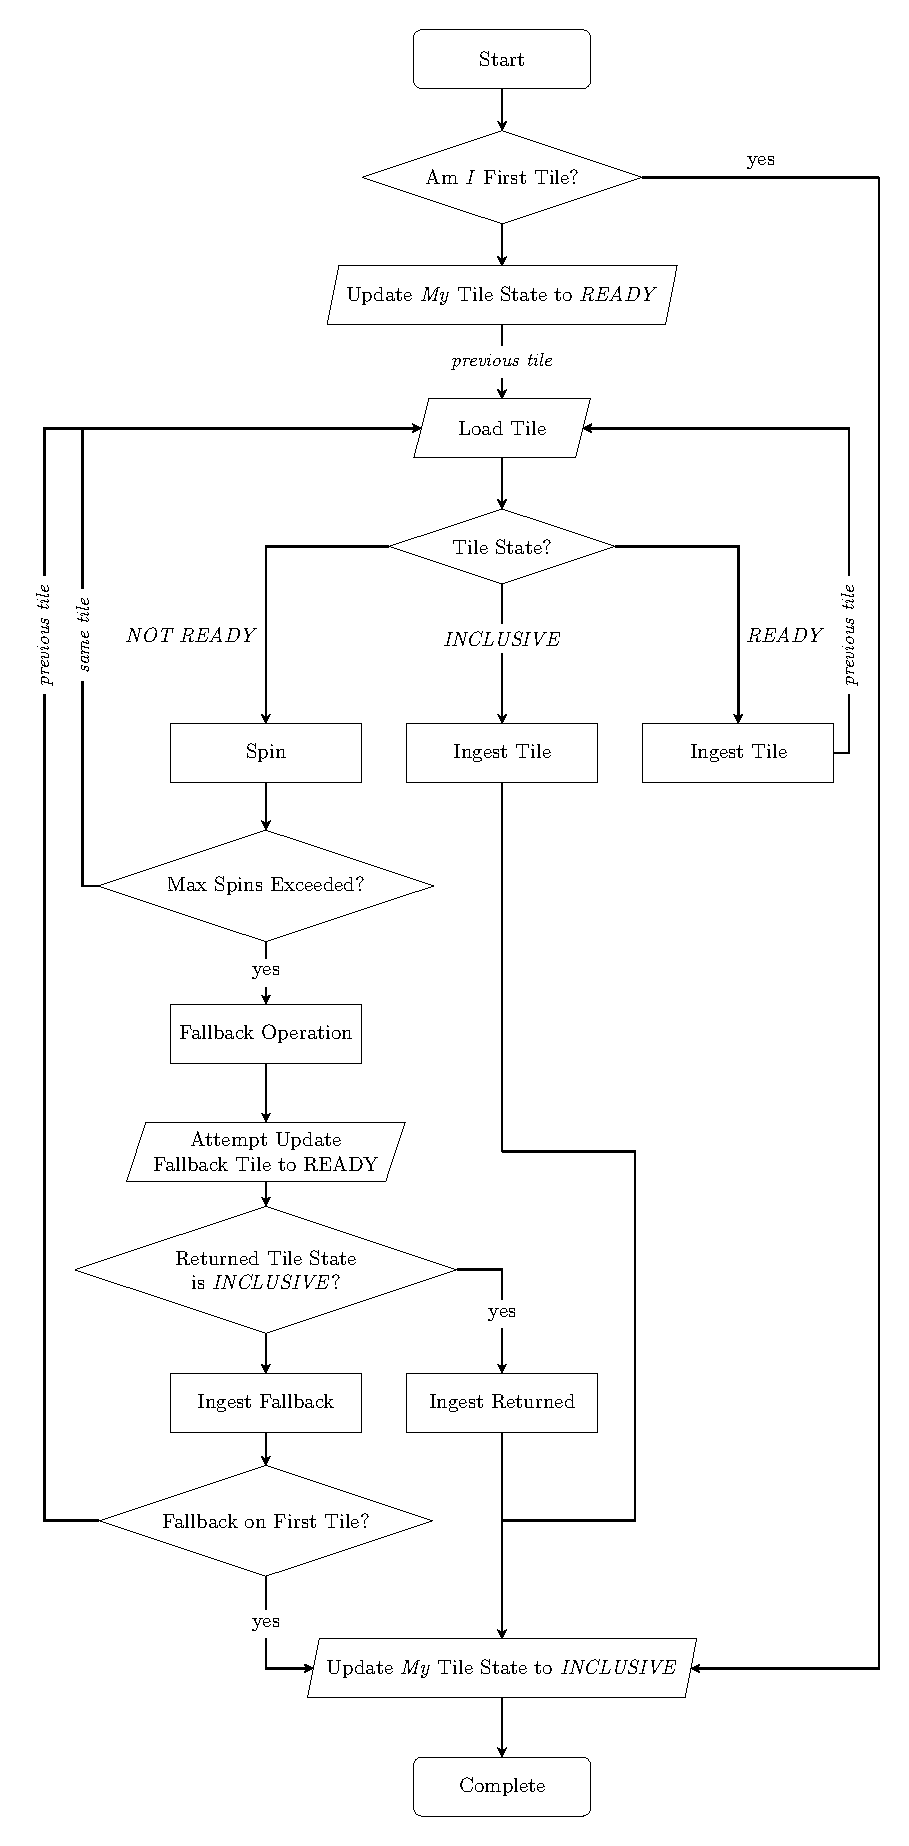
\includegraphics[width=\linewidth]{graphics/FlowChart.pdf}
  \label{fig:decoupled_fallback}
  \caption{Flow Chart Representation of Decoupled Fallback}
\end{figure}
\begin{enumerate}
  \item[(0)] \textbf{Posting Local Reduction:}
        \begin{itemize}
          \item Each workgroup posts its local reduction---the result of the workgroup-wide scan over partials---to global memory and updates its tile state to \emph{Ready}.
          \item If it is the first work tile, its local reduction \emph{is} its inclusive reduction. In this case, the workgroup updates its tile state directly to \emph{Inclusive} and bypasses the \emph{Chained-Propagation} phase entirely.
        \end{itemize}

  \item \textbf{Initialization:}
        \begin{itemize}
          \item The control flag, initialized to \emph{Locked}, signals that the workgroup should enter the \emph{Chained-Propagation} phase.
          \item The first thread initializes a \emph{previous reduction} variable in registers with $\varepsilon$ to hold the accumulated reductions of preceding tiles.
          \item The first thread initializes a \emph{current tile} pointer to its immediate predecessor, with which it begins to traverse backwards through the spine.
        \end{itemize}

  \item \textbf{Lookback:}
        \begin{itemize}
          \item The first thread queries the state of \emph{current tile}.
                \begin{itemize}
                  \item If the tile is in the \emph{Ready} state, the workgroup ingests the value and sets \emph{current tile} to the preceding tile, repeating this step until reaching a tile that is \emph{Not Ready}.
                  \item If the tile is in the \emph{Inclusive} state, the workgroup ingests the value and proceeds directly to step~4.
                  \item If the tile is in the \emph{Not Ready} state, the first thread spins for a limited number of iterations, defined by the \emph{Maximum Spin Count}.
                        \begin{itemize}
                          \item If this count is exceeded, it exits the lookback loop and proceeds to step~3, leaving the control flag \emph{Locked} to signal to the workgroup that a fallback is required. Additionally, it copies \emph{current tile} into shared memory to broadcast the fallback tile identity to the workgroup.
                          \item Otherwise, it continues spinning until the tile transitions to a \emph{Ready} or \emph{Inclusive} state. Without FPG, \emph{Decoupled Lookback} risks spinning indefinitely and deadlocking at this stage.
                        \end{itemize}
                \end{itemize}
        \end{itemize}

  \item \textbf{Fallback:}
        \begin{itemize}
          \item If the blocking tile is still \emph{Not Ready} after waiting, the workgroup initiates a fallback operation.
          \item Using the tile index provided by the first thread, the full workgroup computes the reduction of the blocking tile by directly processing the corresponding elements. This process involves a \emph{workgroup-wide reduction},\footnote{See footnote NUMBER.} utilizing additional shared memory to aggregate partial subgroup results.
          \item Once the fallback reduction is complete, the workgroup \emph{attempts} to post the reduction to global memory and update the tile's state to \emph{Ready}.
          \item As this update attempt is performed atomically, the workgroup simultaneously reads back the blocking tile's most recent state:
                \begin{itemize}
                  \item If that most recent state is \emph{Inclusive}, the fallback value computed by the workgroup is discarded, and the first thread ingests the returned value before proceeding to step 4.
                  \item Otherwise, the first thread ingests the fallback value.
                        \begin{itemize}
                          \item If the blocking tile is the first in the spine, the workgroup has reached the start of the spine and has thus completed the \emph{Chained Propagation}. The first thread proceeds to step 4.
                          \item Otherwise, the first thread updates \emph{current tile} to the preceding tile, returning to the lookback process in step~2.
                        \end{itemize}
                \end{itemize}
        \end{itemize}

  \item \textbf{Finalization:}
        \begin{itemize}
          \item To prioritize inter-workgroup reduction propagation, the first thread immediately adds the local reduction to \emph{previous reduction}, posts the inclusive reduction to global memory, and transitions the tile state to \emph{Inclusive}.
          \item It then writes \emph{previous reduction} to shared memory, allowing all threads to combine it with their \emph{workgroup-wide} and private scan computations.
          \item Finally, the first thread sets the control flag to \emph{Unlocked}, signaling the rest of the workgroup that \emph{Chained Propagation} has completed, and allowing the final write phase to begin.
        \end{itemize}
\end{enumerate}

\subsection{Tile State Implementation}
In all variants of \emph{Chained-Scan}, there is communication and synchronization between workgroups. The fundamental primitive is \emph{message passing,} meaning that one workgroup posts the result of a communication, then other workgroups read it. This primitive is well studied in the context of memory models~\cite{}. \raph{The earliest publication of the MP litmus test appears to be section 2.1 of "Intel 64 Architecture Memory Ordering White Paper". I'm not sure that's the best cite; the MC mutants paper cites https://arxiv.org/pdf/1207.7264} The key requirement is both control synchronization, meaning the reader does not proceed until the writer sends the message; and data synchronization, meaning that the reader reads the correct value. The latter is especially challenging in relaxed memory models as are employed on GPUs.

Combined control and data synchronization can be accomplished by packing both the tile state and the reduced value into a single word, using relaxed atomic store to send the message, and relaxed atomic load to receive the message, spinning as necessary until the tile state is updated. The semantics of atomics guarantee, even with relaxed memory ordering, that the data is fresh. However, if the tile state and data are stored in two different memory locations, then relaxed atomics are not sufficient and some other sychronization is necessary. On CPUs, it is common to upgrade the memory semantics from relaxed to acquire/release, which then provides the necessary guarantee. \raph{Here's a good place to cite the MP litmus test because that's exactly what it's about.} Unfortunately, on GPUs, acquire/release semantics are neither portable (they are only available on Vulkan, and optional until version 1.3), nor are they necessarily efficient even when they are available; often the implementation involves expensive cache flushes. A device-scoped memory barrier has similar problems. While it would provide the necessary guarantee, it is also not available in WebGPU (or in versions of Metal prior to 3.2), and is expensive.

Without some other mechanism, the requirement to pack tile state and data into a single word limits the data to 30 bits (assuming 2 bits for the tile state). That, in turn, makes it impossible to represent common ordinary 32-bit floating point values without loss of precision. While some GPUs support 64 bit atomics (and it is likely that WebGPU will include them as an optional extension), that is also sadly not portable, and merely raises the payload limit to 62 bits without eliminating it altogether.

A key innovation of this paper is to \emph{split} the reduced values into multiple atomics, each carrying its own copy of the tile state. The message is received when relaxed atomic loads of all the parts agree on their tile state. This way, the payload is reconstructed intact, even in the absence of any guarantees from the memory model stronger than relaxed atomics.

In particular, we use two or four 32-bit values, splitting the reduction value into 16-bit segments while reserving the two most significant bits of each 32-bit value to encode the tile state.
\begin{figure}[h!]
  \centering
  \includegraphics[width=\linewidth]{graphics/split.pdf}
\end{figure}

To accommodate the split values during \emph{Chained Propagation}, we use two or four threads from the first subgroup, leveraging subgroup \emph{ballot} to verify state consistency, and subgroup \emph{shuffle} to join and split reductions. With one thread per 16 bits and a minimum subgroup size of four in WebGPU, this method supports both 32-bit and 64-bit values, enabling 64-bit scans without 64-bit atomics or fences.\footnote{Although native 64-bit values are not currently supported by the WebGPU specification, their future inclusion is anticipated.}

Fallbacks require a tile state representation and an atomic operation that can safely transition a tile to \emph{Ready} without overwriting a more advanced state. When an update attempt is made, a blocking tile may be in any of the three states due to either of two scenarios: (1) a false-positive fallback on a tile that transitions to \emph{Ready} or \emph{Inclusive} before fallback completion, or (2) another workgroup completing its fallback first, leaving the tile in \emph{Ready}. If the tile state is \emph{Inclusive} then the write must be skipped, especially because races in writes for the parts may leave the tile permanently in an unreadable state. Thus, a simple atomic store is not suitable. An atomic compare-and-swap would have the correct semantics, but WebGPU lacks this primitive (it does have \texttt{atomicCompareExchangeWeak}, which could possibly be made to work but makes reasoning about correctness and performance more difficult). Instead, we encode the tile state in the most significant bits of the atomic value and enforce a strict state ordering: \emph{Inclusive} $>$ \emph{Ready} $>$ \emph{Not Ready}. This allows an \texttt{atomicMaximum}, which successfully updates to a more advanced state but prevents a state regression, to correctly perform updates.

The atomic splitting technique generalizes to monoids of arbitrary size.

\section{Evaluation}
\subsection{Experimental Setup}
We configure workgroups with a size $w = 256$ threads, where each thread processes $p = 4$ vectors of size 4, resulting in 16 elements per thread and a total work tile size of $t = 4096$. Through testing, \john{across all devices (?)} we find a maximum spin count of 4 effectively balances responsiveness to blocking while minimizing false-positive fallbacks. As the size of the local spine is inversely proportional to the subgroup size, we allocate sufficient shared memory to accommodate the WebGPU standard's minimum subgroup size of 4. Due to our overall thriftiness with shared memory, total usage remains modest at only $\sim$1 KB\@. For all tests, we use an input size of $2^{25}$ \john{It would be worthwhile, I think, to run a test against CUB where the x axis is problem size and the y axis is throughput. A reviewer might think we're hiding something if we only report results for one (large) input size. I imagine that our performance will look similar to CUB's at all input sizes and that is the result we want.} and an inclusive prefix sum. Our test hardware, listed POSITIONAL-RELATION, spans a wide range of FPG and performance capabilities. We empirically find that the Google Chrome native implementation of WebGPU (Dawn) provides the best performance and use it for all testing, except on the Arm-Mali GPU, which requires Android native, necessitating the use of WGPU\@.\footnote{To keep the perforamance as close to Dawn as possible, we translate our WGSL code with Dawn's Tint transpiler, and provide the raw SPIR-V to WGPU\@.}
\begin{table}
  \centering
  \small
  \begin{tabular*}{\linewidth}{@{\extracolsep{\fill}} l l c r r}
    \toprule
    Vendor & Device Name & OBE? & Occupancy & Subgroup Size \\
    \midrule
    Intel  & HD Graphics 620       & \textbf{Yes} & 9   & 8--32  \\
    ARM    & Mali-G78 MP20          & \textbf{Yes} & 40  & 16  \\
    Apple  & M1 Pro Max             & \textbf{No}  & 64  & 32  \\
    NVIDIA & GeForce RTX 2080 Super & \textbf{Yes} & 192 & 32  \\
    AMD    & Radeon RX 7900 XT      & \textbf{Yes} & 420 & 32--64  \\
    \bottomrule
  \end{tabular*}
  \caption{Hardware Specifications of Testing Devices.}
  \label{tab:hardware}
\end{table}

\subsection{Performance Comparison}
\subsubsection{Performance Versus Contemporary Implementations:}
We first compare \emph{Decoupled Fallback} (\emph{CSDLDF}) to \emph{Decoupled Lookback} (\emph{CSDL}) in NVIDIA’s \emph{CUB} library\footnote{CUDA toolkit 12.8, CUB/CCCL VERSION}~\cite{}. As this test is limited to CUDA, evaluation is restricted to the 2080 Super. Due to WebGPU’s 128MB storage buffer limit, we test input sizes from $2^{10}$ to $2^{25}$\!.

To isolate the effect of \emph{Decoupled Fallback}, we implement our own \emph{CSDL} with an identical local-scan implementation. Our \emph{CSDL} implementation outperforms \emph{CUB} before reaching saturation, and likely due to this advantage, \emph{CSDLDF} achieves near-identical performance to \emph{CUB} despite its additional \emph{Chained-Propagation} overhead. While Dawn struggles, it still reaches saturation at larger inputs. However, cross-API comparisons remain challenging, as despite nearly identical high-level code, all implementations perform significantly better in CUDA, particularly for inputs smaller than $2^{20}$\!, where CUDA more effectively utilizes the 2080 Super’s 4MB L2 cache.

\begin{figure}
  \centering
  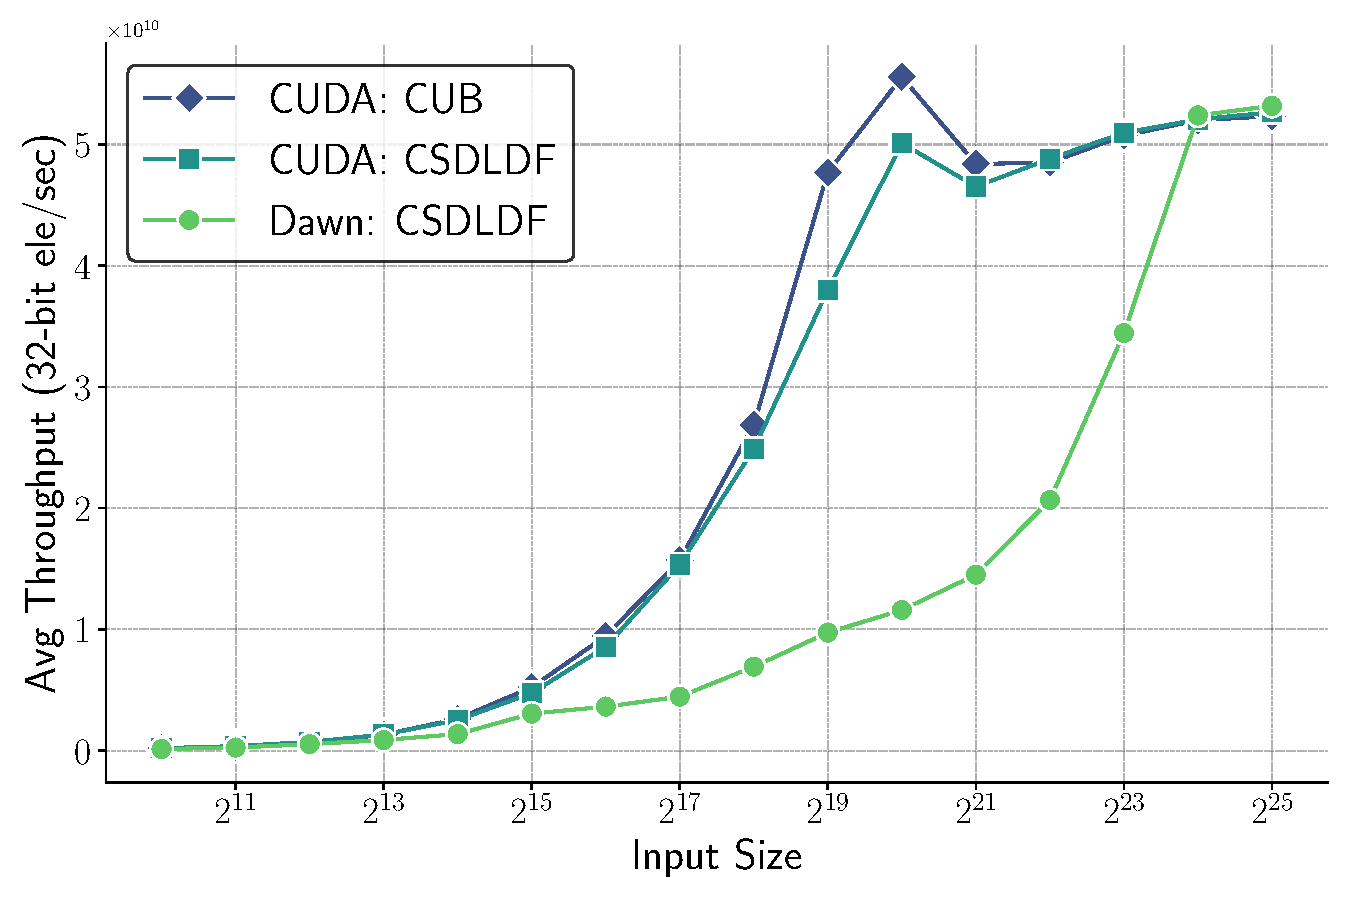
\includegraphics[width=\linewidth]{graphics/cuda_plot.pdf}
\end{figure}

\subsubsection{Same-API Performance Versus Baseline Measures}
To evaluate the performance of \emph{Decoupled Fallback} (\emph{CSDLDF}), we compare it against two key benchmarks: \emph{Memcopy}\textdagger{~\ref{sec:memcopy}} and \emph{Reduce then Scan}\textdagger{~\ref{sec:rts}} (\emph{RTS}). \emph{RTS} serves as a baseline to demonstrate the performance gains of our approach over the previous FPG-constrained technique. \emph{Memcopy} is included as a point of reference, as it shares the same $2n$ global memory movement as \emph{Decoupled Fallback}, without any compute overhead and thus is guaranteed to be memory bandwidth bound. \john{Nit: I would use \texttt{memcpy} as the name of this benchmark to match how it's actually called in C etc.}

\begin{table*}
  \centering
  \begin{tabular*}{\textwidth}{@{\extracolsep{\fill}} l r r r r r}
    \toprule
    Metric & Intel HD620 & ARM Mali-G78 MP20 & Apple M1 Pro Max & Nvidia 2080 Super & AMD 7900 XT \\
    \midrule
    H-Mean \emph{Memcopy} (32-bit ele/sec)  & 1.498e9   & 106.663e9 & 54.203e9  & 54.203e9  & 71.190e9  \\
    H-Mean \emph{CSDLDF} (32-bit ele/sec)   & 1.487e9   & 112.430e9 & 53.256e9  & 53.256e9  & 95.737e9  \\
    H-Mean \emph{RTS} (32-bit ele/sec)      & 1.060e9   & 82.302e9  & 35.709e9  & 35.709e9  & 62.868e9  \\
    \emph{CSDLDF}/\emph{Memcopy} (\%)       & 99.2\%    & 105.4\%   & 98.3\%    & 98.3\%    & 134.5\%   \\
    \emph{CSDLDF}/\emph{RTS} (\%)          & 140.2\%   & 136.6\%   & 149.1\%   & 149.1\%   & 152.3\%   \\
    Avg Spins per Wg    & 0.306    & 1.380    & 0.418    & 0.418    & 0.133    \\
    Avg Lookback Length per Wg  & 1.725    & 3.510    & 13.139   & 13.139   & 20.867   \\
    Avg Total Fallbacks Initiated      & 260.364   & 2202.045  & 88.384   & 88.384   & 10.127   \\
    Avg Total Successful Insertions    & 6.084     & 57.875    & 1.205    & 1.205    & 1.001    \\
    \bottomrule
  \end{tabular*}
  \caption{MALI ABSOLUTE SPEED WRONG!, \emph{Decoupled Fallback} performance, 32-bit Inclusive Prefix Sum, Input Size $\mathbf{2^{25}}$. \john{I would label metrics as ``H-Mean \emph{Memcopy} (32-bit ele/sec $\cdot 10^9$)'' and then leave the exponents out of the main table.}\john{Separately, h-mean is the right summary statistic \emph{if} the distribution is Gaussian, which it almost certainly is not. Like most measurements of this type, it's much more likely log-normal. I am influenced here by \url{https://lemire.me/blog/2023/04/06/are-your-memory-bound-benchmarking-timings-normally-distributed/}.}\john{I note Apple and NVIDIA timings are identical, but figure you know that.}}
  \label{tab:results}
\end{table*}

As shown in Table~\ref{tab:results}, with the exception of the ARM Mali, \emph{CSDLDF} achieves at least a $\sim$40\% speedup over \emph{RTS} across all tested devices. Since \emph{Memcopy} is purely memory bandwidth bound, \emph{CSDLDF} should ideally match its throughput. This holds across most devices, except for the AMD 7900 XT, where \emph{CSDLDF} slightly outperforms \emph{Memcopy}, suggesting improved memory structuring due to compute operations. \john{I have no idea what this previous phrase means.} On the ARM Mali, \emph{CSDLDF} appears to underperform, achieving only a 36\% speedup instead of the expected 50\%. However, as its performance is nearly identical to \emph{Memcopy}, this indicates that the implementation is memory-bandwidth-bound, limiting further gains.

\subsection{How (un)fair is fair?}
Show the stats of each device. How many lookbacks?  How many fallbacks initiated? How many successful fallbacks?

\subsection{Simulated Blocking}
To demonstrate the resilience of our technique under fallback rates significantly higher than those observed organically on devices, we intentionally force fallbacks by omitting the posting of work tile reductions. Starting with infrequent omissions---1 in 512 workgroups---we progressively increase the rate to near-continuous levels, reaching 1 in 2 workgroups.
\begin{figure*}[t]
  \centering
  \begin{subfigure}[t]{0.48\linewidth}
    \centering
    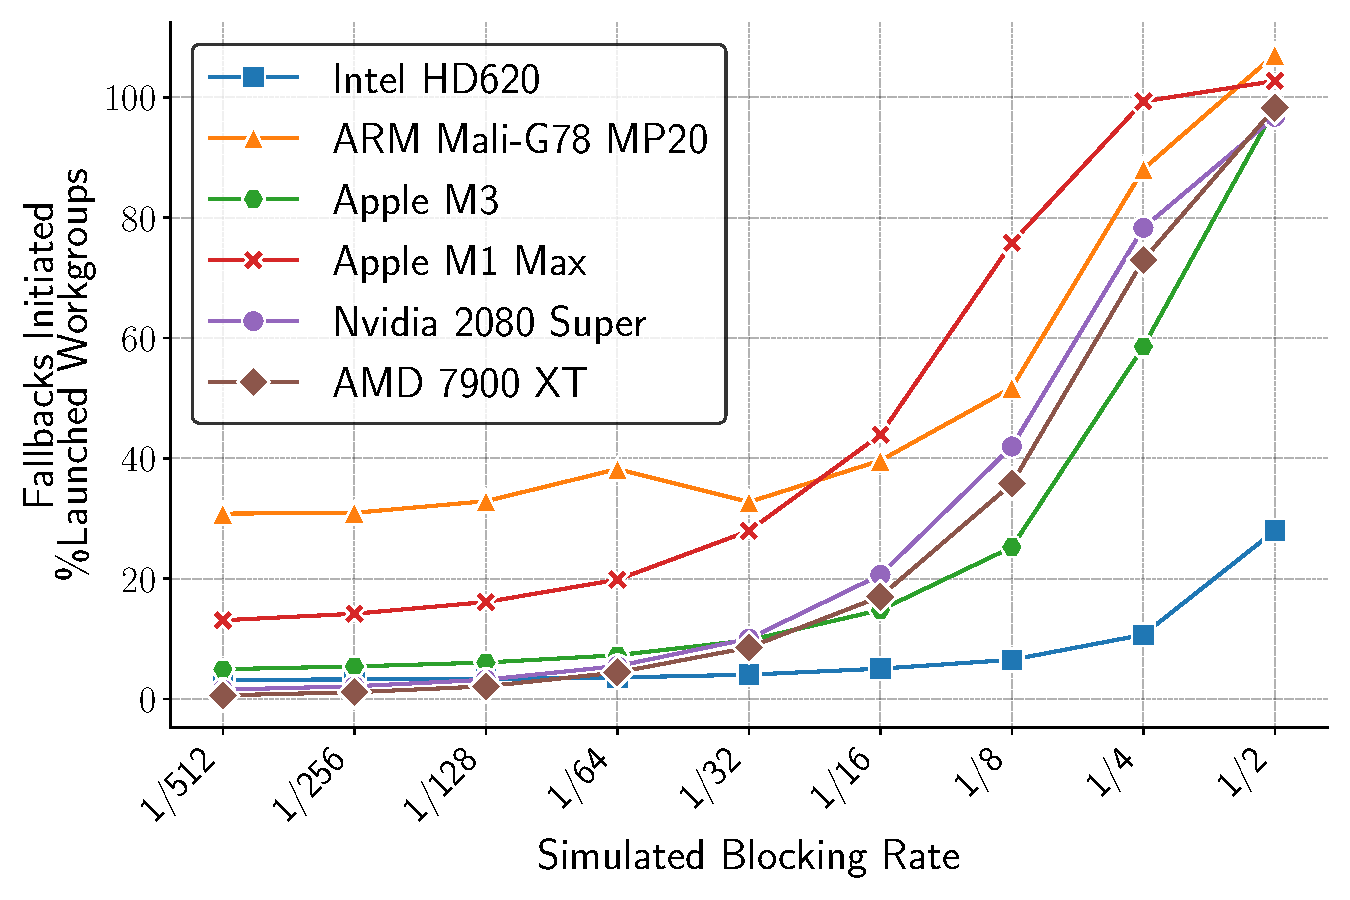
\includegraphics[width=\linewidth]{graphics/fallbacksInitiated_plot.pdf}
    \caption{Fallbacks Initiated}
    \label{fig:fallbacks_initiated}
  \end{subfigure}\hfill
  \begin{subfigure}[t]{0.48\linewidth}
    \centering
    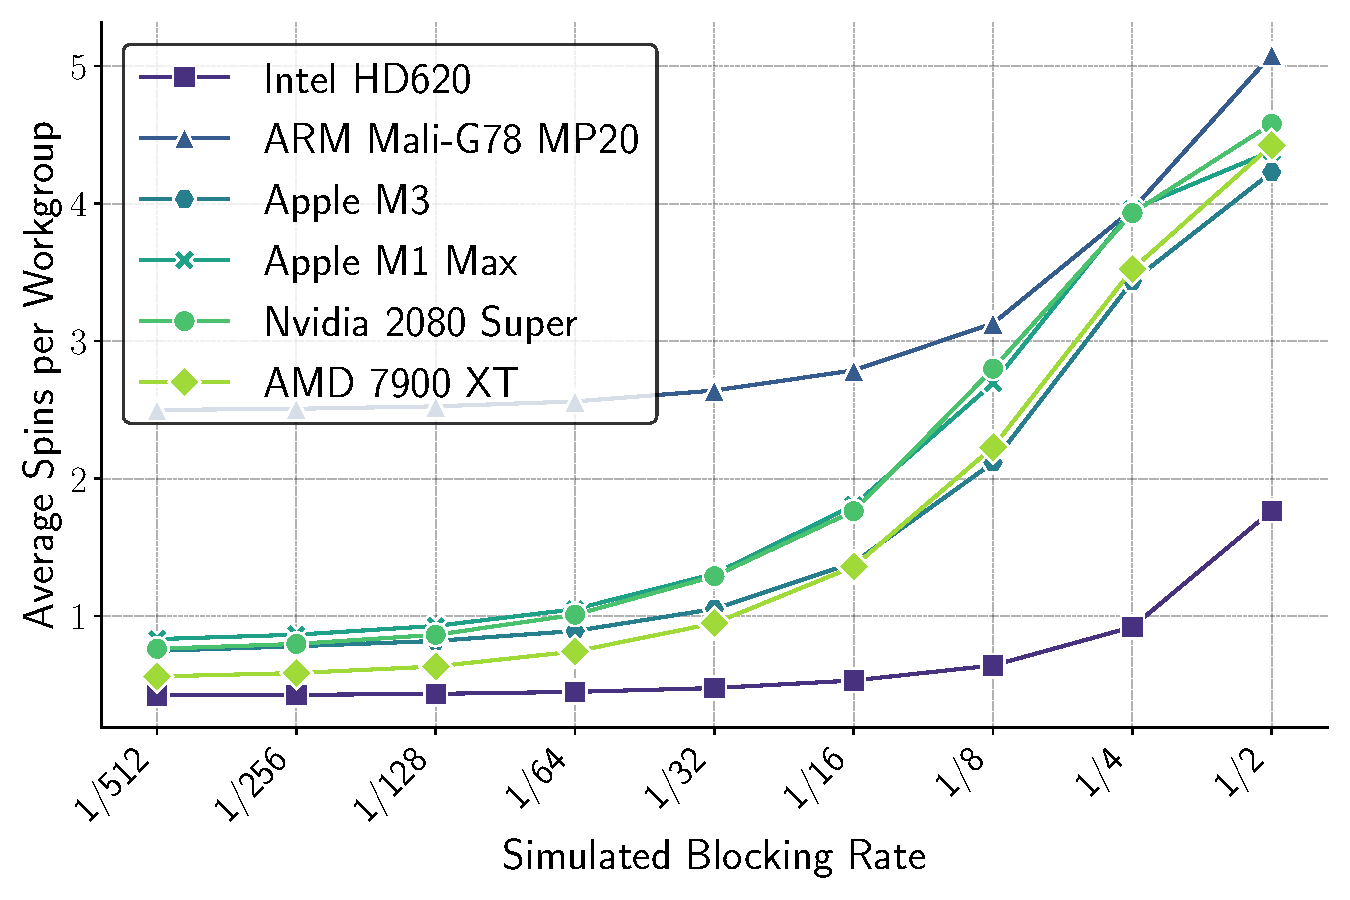
\includegraphics[width=\linewidth]{graphics/totalSpins_plot.pdf}
    \caption{Total Spins}
    \label{fig:total_spins}
  \end{subfigure}

  \vspace{0.2em}

  \begin{subfigure}[t]{0.48\linewidth}
    \centering
    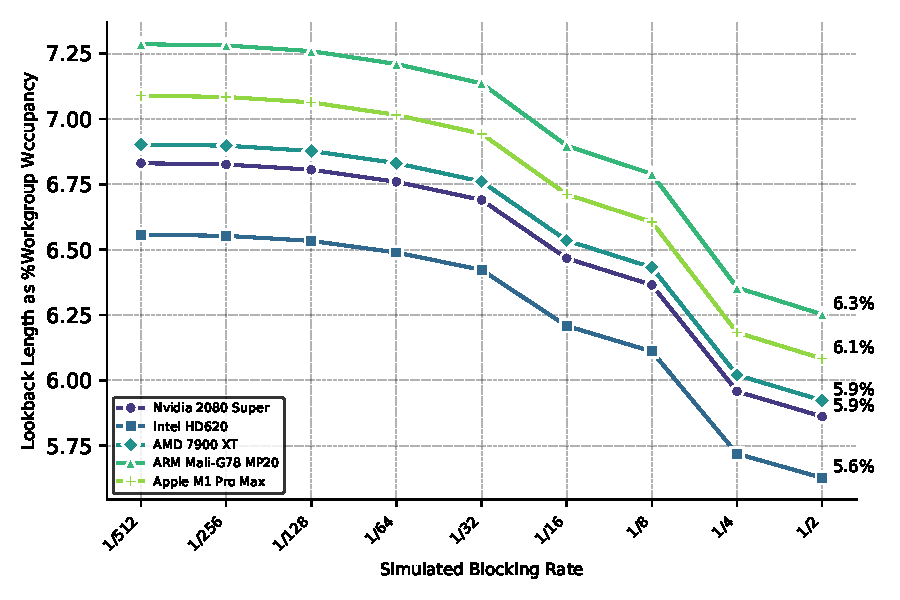
\includegraphics[width=\linewidth]{graphics/lookbackLength_plot.pdf}
    \caption{Lookback Length}
    \label{fig:lookback_length}
  \end{subfigure}\hfill
  \begin{subfigure}[t]{0.48\linewidth}
    \centering
    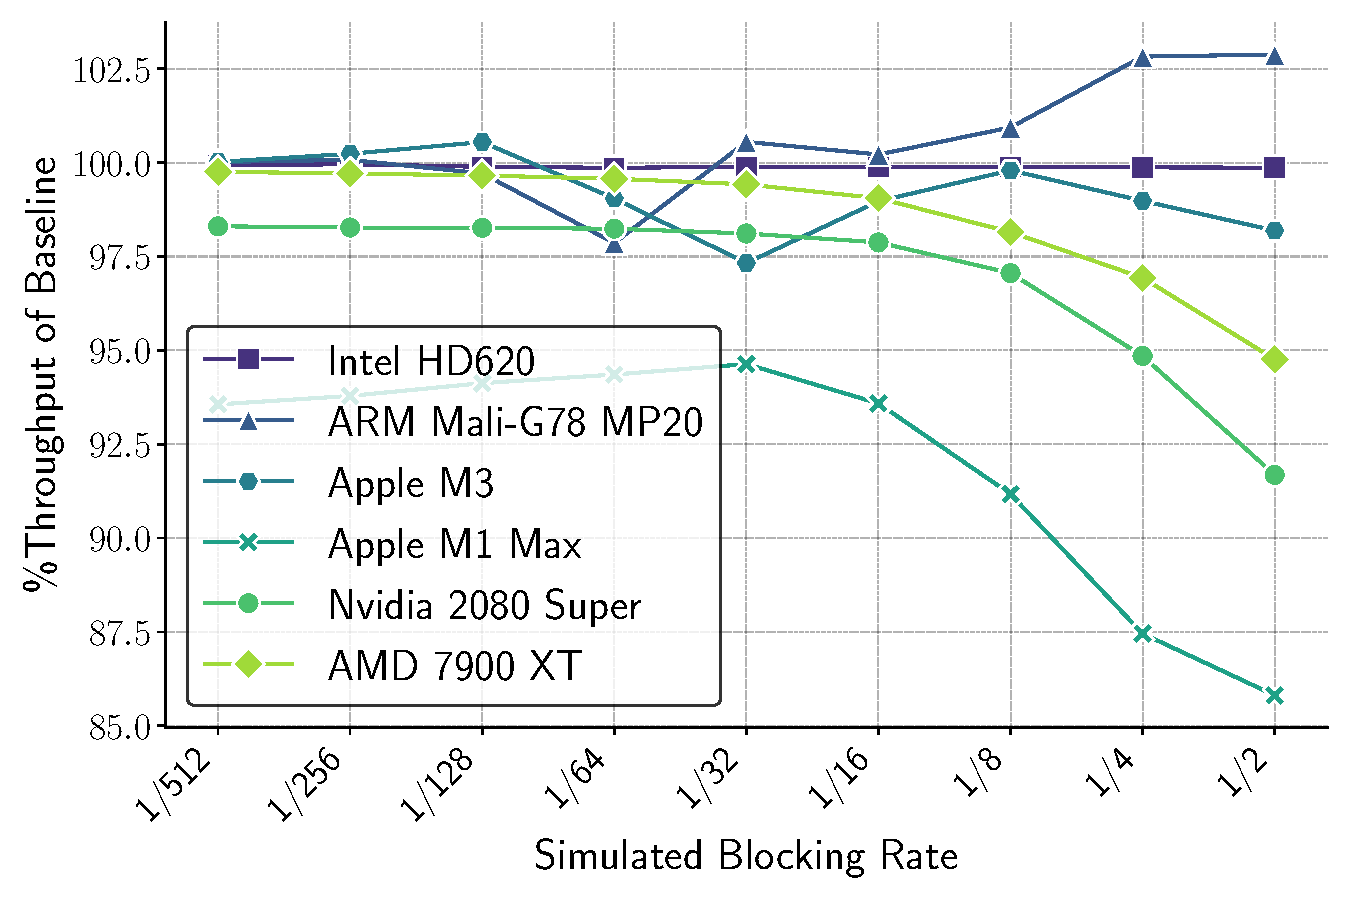
\includegraphics[width=\linewidth]{graphics/time_plot.pdf}
    \caption{Throughput vs Baseline}
    \label{fig:execution_time}
  \end{subfigure}

  \caption{Simulated Blocking}
  \label{fig:vertical_images}
\end{figure*}

In Figure~\ref{fig:fallbacks_initiated}, we measure the number of fallbacks proportional to the number of workgroups launched, and verify that we are indeed inducing fallbacks. In Figure~\ref{fig:total_spins} we measure \thomas{this should be spins per workgroup it's a better metric}. In Figure~\ref{fig:lookback_length} we see that. Finally, in Figure~\ref{fig:execution_time}, we can see that, even when \emph{half} the workgroups are deadlocking, \emph{Decoupled-Fallback} still achieves speeds of . . .

\section{Discussion}

\subsection{Trade-offs}

\subsection{Limits on Speed-of-Light Performance}
There are a number of factors which may preclude speed-of-light performance, but most salient is the fairness of the scheduling model. In \emph{Decoupled-Fallback}, a work tile which is late due to unfairness is indistinguishable from one which is blocking, so as a scheduler becomes increasingly unfair, it incurs an increasing number of redundant fallbacks. Consider a hardware with a workgroup occupancy denoted by $o$, and let $f$ represent the probability that a fallback operation occurs at a particular lookback step. Because the number of lookback steps is bounded by $o$, the expected number of fallback operations is approximately $fo$. This results in a factor of $fo$ increase in global memory reads and a factor of $fo\log{n}$ increase in work.

This increased sensitivity to fairness exacerbates existing issues which negatively impact the performance of previous scan architectures, namely lack of compute, and slow atomic update latency. On hardware that lacks sufficient compute power to be memory-bandwidth bound, the additional work incurred by redundant fallback reductions is particularly deleterious. High atomic update latency further compounds the problem: as inter-workgroup communication time grows, the minimum delay before updates become visible to dependent workgroups also increases. This, in turn, raises the number of lookback steps that may be needed and potentially leads to redundant fallbacks.

\thomas{Somewhere in here is perfect for Raph's commentary on the speed of atomics on different hardware. Once we have it, we can retool this section around it.}

\begin{acks}
\end{acks}

\clearpage
\appendix
\section{Artifact}
\subsection{Baseline Comparisons: \emph{Memcopy}}
\label{sec:memcopy}
\begin{table}[h!]
  \small
  \centering
  \begin{tabular}{l r r}
    \toprule
    Device & \makecell{Memory \\ Bandwidth \\ (GB/s)} & \makecell{Expected \\ Throughput \\ (32-bit ele/sec)} \\
    \midrule
    Intel HD620 (Single-/Dual-Channel) & 17.1 / 34.1  & 2.13e9 / 4.26e9 \\
    ARM Mali-G78 MP20 / Pixel 6a (Tensor) & 51.2  & 6.40e9 \\
    Apple M1 Pro Max   & 200  & 25.0e9 \\
    Nvidia 2080 Super  & 496  & 62.0e9 \\
    AMD 7900 XT        & 800  & 100.0e9 \\
    \bottomrule
  \end{tabular}
  \caption{Vendor-Specified Memory Bandwidth and Expected Throughput (32-bit Elements per Second)}
  \label{tab:memory_bandwidth}
\end{table}
Although all backend APIs support \emph{timestamp queries inside encoders}, Apple GPUs do not, so we are forced to implement our own \emph{Memcopy} kernel to measure memory bandwidth, as opposed to simply timing an API's copy buffer operation. It is well known that \emph{observed} peak memory bandwidth, tends to diverge from vendor-listed peak bandwidth, so for completeness we list these figures above. We make a number of observations:
\begin{itemize}
  \item \textbf{Intel HD620:} As our HD620 laptop is only equipped with a single memory DIMM, its peak bandwidth is limited to the lower bound, 2.13e9 ele/sec. Thus, our observed bandwidth of 1.498e9 is reasonable.
  \item \textbf{ARM Mali-G78 MP20 / Pixel 6a (Tensor):} The observed throughput is significantly lower than expected, despite a vendor-listed bandwidth of 6.40e9 ele/sec. The cause of this discrepancy remains unclear, but we note other developers have observed similar speeds.
  \item \textbf{Apple M1 Pro Max:} Observed throughput matches expectations.
  \item \textbf{Nvidia 2080 Super:} Observed throughput matches expectations.
  \item \textbf{AMD 7900 XT:} Our above result, where \emph{CSDLDF} was observed to be faster than \emph{Memcopy}, is likely due to compute latency counterintuitively improving memory access patterns, leading to reduced paging. Furthermore, we see that our \emph{CSDLDF} throughput is within spec and reasonable.
\end{itemize}

\subsection{Baseline Comparisons: \emph{Reduce then Scan}}
\label{sec:rts}
As we desire the most competitve baseline possible, our \emph{RTS} kernels employ the same intra-workgroup scan strategy and tuning parameters as \emph{CSDLDF}. Initially, we adopted Merrill and Grimshaw's~\cite{Merrill2009} workgroup raking approach for inter-workgroup processing. However, empirical testing revealed that raking was consistently outperformed—by up to $\sim$15\% on lower-end devices—by a simpler approach that processes the spine serially with a single workgroup. Furthermore, our \emph{RTS} performance closely aligns with the theoretically expected $O(3n)$ global memory movement.

\subsection{Availability}
We provide our artifact in the following GitHub repository:
\thomas{Will anonymize with GithubAnonymous once we are ready.}

\subsection{Requirements}

\subsubsection{Device Requirements}
Any device supporting Dawn, with subgroup and timestamp query capabilities, and at least 384 MB of available device memory. Requires at least $\sim$2GB of disk memory to build Dawn.

\subsubsection{Software Requirements}
\begin{itemize}
  \item Git
  \item CMake 3.10.2+ or another C++ build tool
  \item C++17-compliant compiler (Clang recommended)
  \item Python for fetching dependencies
\end{itemize}

\subsection{Building}
Although native WebGPU is supported on various operating systems—most notably Windows, macOS, and Linux—this section will focus on building it in Unix-like environments for the sake of brevity, using CMake as the example build tool, and Clang++ as the example compiler.

\subsubsection{Building Dawn}
\begin{enumerate}
  \item[(0)] Dawn depends on the following packages (Ubuntu package names):
  \begin{lstlisting}[basicstyle=\ttfamily\small, frame=single]
sudo apt install libxrandr-dev \
  libxinerama-dev libxcursor-dev libxi-dev \
  libx11-xcb-dev mesa-common-dev
  \end{lstlisting}

  \item Clone the Dawn repository:
  \begin{lstlisting}[basicstyle=\ttfamily\small, frame=single]
git clone https://dawn.googlesource.com/dawn
cd dawn
git fetch --all
git checkout chromium/6950
  \end{lstlisting}

  \item Build and install Dawn:
  \begin{lstlisting}[basicstyle=\ttfamily\small, frame=single]
cd dawn
cmake -S . -B out/Release \
  -DDAWN_FETCH_DEPENDENCIES=ON \
  -DDAWN_ENABLE_INSTALL=ON \
  -DCMAKE_BUILD_TYPE=Release \
  -DDAWN_BUILD_TESTS=OFF \
  -DDAWN_BUILD_SAMPLES=OFF \
  -DTINT_BUILD_TESTS=OFF \
  -DTINT_BUILD_CMD_TOOLS=OFF \
  -DCMAKE_CXX_COMPILER=clang++

cmake --build out/Release \
  --parallel <num_threads>

cmake --install out/Release \
  --prefix install/Release
  \end{lstlisting}
\end{enumerate}

\subsubsection{Building Artifact}
After successfully building and installing Dawn, follow these steps to build the artifact:

\begin{enumerate}
  \item Navigate to the artifact directory:
  \begin{lstlisting}[basicstyle=\ttfamily\small, frame=single]
cd Decoupled-Fallback-Paper/artifact/Dawn
  \end{lstlisting}

  \item Set the `CMAKE\_PREFIX\_PATH` to point to your Dawn installation directory:
  \begin{lstlisting}[basicstyle=\ttfamily\small, frame=single]
export CMAKE_PREFIX_PATH=/path/to/dawn/ \
  install/Release
  \end{lstlisting}

  \item Build the artifact:
  \begin{lstlisting}[basicstyle=\ttfamily\small, frame=single]
cmake -S . -B out/Release \
  -DCMAKE_BUILD_TYPE=Release \
  -DCMAKE_CXX_COMPILER=clang++
  \end{lstlisting}

  \item Compile the project:
  \begin{lstlisting}[basicstyle=\ttfamily\small, frame=single]
cmake --build out/Release
  \end{lstlisting}
\end{enumerate}

\subsubsection{Running the Artifact}
Once the artifact has been successfully built, you can run it using the following command:

\begin{lstlisting}[basicstyle=\ttfamily\small, frame=single]
./out/Release/dawn <TestType> [record] [deviceName]
\end{lstlisting}

where:
\begin{itemize}
    \item \texttt{<TestType>} specifies the test to run. Valid options are:
    \begin{itemize}
        \item \texttt{csdl} – Runs the \emph{Decoupled Lookback} test. \textbf{Warning}, this \emph{will} crash without FPG\@.
        \item \texttt{csdldf} – Runs the \emph{Decoupled Fallback} test.
        \item \texttt{full} – Runs a full set of tests, including multiple \emph{Decoupled Fallback} simulations.
    \end{itemize}
    \item \texttt{record} (optional) enables recording the test results to a CSV file.
    \item \texttt{deviceName} (optional) appends the device name to recorded test results.
\end{itemize}

\bibliographystyle{ACM-Reference-Format}
\bibliography{bib}

\end{document}
\endinput

%%% Local Variables:
%%% mode: LaTeX
%%% TeX-master: t
%%% End:
